\subsection{Artifically Intelligent Agents}
    An Artificial General Intelligence (AGI) would possess at least the capabilities shown in Figure \ref{fig:AIcapabilities}(as the typical human does). At this time AGIs cannot be build, instead highly specialized versions exist, which will be referred to as AIs in this paper. An AI is an agent that possess, to some extent, at least one of the capabilities shown in the figure. This is a very weak notion of AI, but encompasses much of the current systems that are being marketed as artificially intelligent at this time.\footnote{This group of capabilities would generally be accepted in the AI community although it may be necessary to add other categories like imagination, creativity, and social interaction. For this reason the `at least' qualifier was used.}

    The following simple definitions of the AGI capabilities will help to ground further discussion in the paper:

    \begin{description}
        \item [Reasoning (R)]: The ability to solve problems, and make conclusions.
        \item [Knowledge Representation (K)]: The ability to internally represent knowledge of information that has been learned.
        \item [Planning (Pl)]: The ability to make a plan in order to accomplish a goal within an environment.
        \item [Learning (L)]: The ability to learn from experience and data.
        \item [Perception (Pe)]: The ability to use different sensors to perceive the surrounding environment.
        \item [Motion/Manipulation (M)]: The ability to move within an environment and manipulate parts of it.
        \item [Interaction (I)]: The ability to interact with other intelligent agents. For communicating with humans this could involve some type of natural language interface.
    \end{description}

    The research discipline called machine learning (ML) is a subset of the AI research landscape. Individual ML algorithms might be thought of as being a highly specialized AI that is contained within only one of the AGI capabilities.

	\begin{figure}[htbp]
    	\centering
     	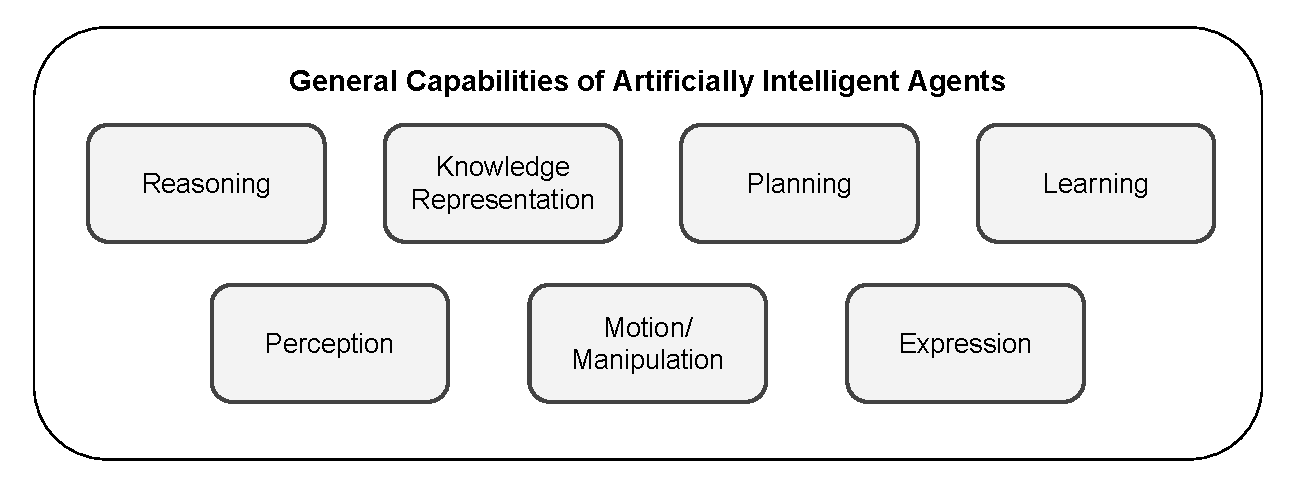
\includegraphics[width=0.9\textwidth]{Figures/AI_capabilities}
    	\caption{List of the capabilities of an artificial general intelligence. In this paper an AI is defined as a system that possesses at least one of the capabilities illustrated.}
        \label{fig:AIcapabilities}
    \end{figure}

    Concretely, the following systems currently exist and may possess the listed AI capabilities.
    
    \begin{enumerate}
         \item An unmanned aerial system (UAS) possesses the ability to plan, perceive, and move
         \item A personal assistant might be capable of interaction, learning, and reasoning.
         \item An image classifier might possess the capability to learn image classes from labeled examples and predict the class of never-before-seen new images.
         \item \textbf{More???}
     \end{enumerate}


